\documentclass[a4paper,graphics,11pt]{article}

\usepackage[utf8]{inputenc}
\usepackage[T1]{fontenc}
\usepackage{lmodern}
\usepackage[ngerman]{babel}
\usepackage{amsmath, tabu}
\usepackage{amsthm}
\usepackage{amssymb}
\usepackage{algorithm}
\usepackage{algpseudocode}
\usepackage{mathtools}
\usepackage{setspace}
\usepackage{graphicx,color,curves,epsf,float,rotating}
\usepackage{tikz}
\usepackage{../tikz-uml}
\usetikzlibrary{calc}

\floatname{algorithm}{Algorithmus}

\newcommand\norm[1]{\left\lVert#1\right\rVert}
\newcommand\abs[1]{\left\vert#1\right\vert}

\newcommand\aufgabe[1]{\subsection*{Aufgabe #1}}
\newcommand\aufgabenteil[1]{\subsubsection*{#1}}



\pagestyle{empty}
\begin{document}
\noindent WS 2016/17        \hfill Simon Kaiser, 354692 \\
\null                                     \hfill Philipp Hochmann, 356148 \\
\null                                     \hfill Felix Kiunke, 357322 \\
\null                                     \hfill Giacomo Klingen, 356778 \\
\null                                     \hfill Daniel Schleiz, 356092 \\

\begin{center}
\Large \textsc{Softwaretechnik} \\   % Fach
\large Aufgabenblatt 3                        % Nummer das Blattes, nicht vergessen zu ändern!
\end{center}
\begin{center}
\rule[0.5ex]{\textwidth}{0.6pt}\vspace*{-\baselineskip}\vspace{3.2pt}
\rule[0.5ex]{\textwidth}{1.6pt}\\
\end{center}

\DeclareGraphicsExtensions{.jpg}
%%%%%%%%%%%%%%%%%%%%%%%%%%%%%%%%%%%%%%
%
%   Ab hier kommt der Text
%   Neue Aufgabe mit \aufgabe{}
%   Aufgabenteil mit \aufgabenteil{}
% 
%%%%%%%%%%%%%%%%%%%%%%%%%%%%%%%%%%%%%%

\aufgabe{3.1}

\begin{figure}[h!]
\begin{tikzpicture}
\begin{umlseqdiag}
	\umlobject[class=Kunde]{k}
	\umlobject[class=Mitarbeiter,x=6]{m}
%	\umlobject[class=Pommes,x=11]{p}

	\begin{umlcall}[op=fragtNach(Pommes),dt=5]{k}{m}
		\begin{umlcall}[op=rückfrage(Mayo),return=ja,dt=5]{m}{k}
		\end{umlcall}
		
		\begin{umlcreatecall}[class=Pommes,x=11,op=vorbereiten()]{m}{p}
		\end{umlcreatecall}

		\begin{umlcallself}[op=warten(),dt=6]{k}
		\end{umlcallself}

		\begin{umlcall}[type=return,op=p,dt=6]{p}{m}

			\begin{umlcall}[op={bestellungLiefern(p, mayo)}]{m}{k}
			\end{umlcall}

			\begin{umlcall}[op=essen(schnell)]{k}{p}
			\end{umlcall}

		\end{umlcall}

		\umlsdnode[dt=1,name=end-p]{p}

	\end{umlcall}

	\tikzset{cross/.style={cross out, draw=black, fill=none, minimum size=2*(#1-\pgflinewidth), inner sep=0pt, outer sep=0pt}, cross/.default={2pt}}
	\draw[line width=0.5mm] 
		($ (end-p) - (0.2,0.5) $) -- ++(.4,.4)
		($ (end-p) - (-.2,0.5) $) -- ++(-.4,.4);

\end{umlseqdiag}
\end{tikzpicture}
\end{figure}


\aufgabe{3.2}
\aufgabenteil{a}
W{\"a}hrend Sequenzdiagramme die Interaktion zwischen den einzelnen Objekten zeigen und so eine exemplarische Darstellung von Abl{\"a}ufen und Methodenaufrufen in einem zeitlichen Rahmen erlauben, erlauben Statecharts die Modellierung von Zust{\"a}nden und zeigen den hierarchischen Aufbau des Programms. Diese stellen dann einen m{\"o}glichen Ablauf eines Programms in Verbindung mit den Zust{\"a}nden, die es einnehmen kann dar.
\aufgabenteil{b}
Zun{\"a}chst behandelt der klassische Terminus des Prototyps ein erstes Exemplar oder ein Modell f{\"u}r ein neues Produkt, welches voll funktionsf{\"a}hig, jedoch nicht in Serie anfertigbar ist, in der klassischen Ingenieursdisziplin.\\
In der Softwareentwicklung sind Prototypen jedoch ohne Probleme in Serie fertigbar. Software-Prototypen sind im Gegensatz nicht voll funktionsf{\"a}hig, haben eine kurze Entwicklungszeit und sind preisg{\"u}nstig.\\
Prototyping kann man in in drei Typen klassifizieren: Explorative Prototypen dienen zur Analyse und werden nach Gebrauch verworfen. Experimentelle Prototypen dienen dem Entwickler zur Analyse, Entwurf und auch zur Implementierung. Evolution{\"a}re Prototypen werden innerhalb inkrementeller Entwicklung ausgebaut.
\aufgabe{3.3}
\begin{center}
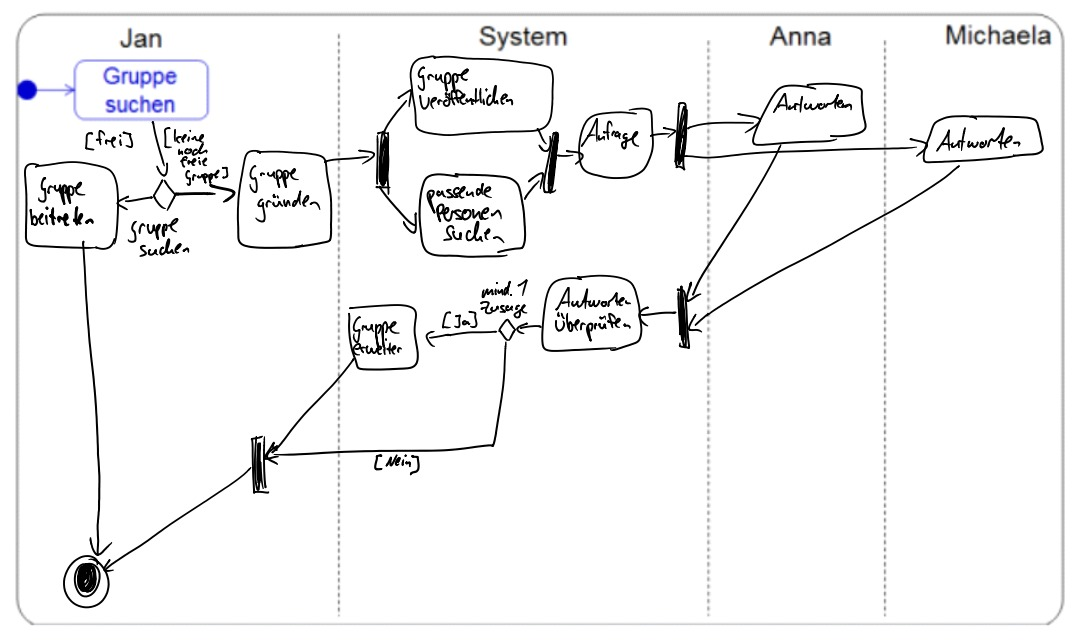
\includegraphics[scale=0.35]{33.jpeg}
\end{center}
\end{document}
% Nummer des Blattes angepasst?
